
%%%%%%%%%%%%%%%%%%%%%%%%%%%%%%%%%%%%%%%%%%%%%%%%%%%%%%%%%%%%%%%%%%%%%
% PREAMBLE
%%%%%%%%%%%%%%%%%%%%%%%%%%%%%%%%%%%%%%%%%%%%%%%%%%%%%%%%%%%%%%%%%%%%%
%
% The following two commands will generate a PDF that follows all the requirements for submission
% and peer review.  Uncomment these commands to generate this output (and comment out the two lines below.)
%
% DOUBLE SPACE VERSION FOR SUBMISSION TO THE AMS
%\documentclass[12pt]{article}
%\usepackage{ametsoc}
%\linenumbers
%
% The following two commands will generate a single space, double column paper that closely
% matches an AMS journal page.  Uncomment these commands to generate this output (and comment
% out the two lines above. FOR AUTHOR USE ONLY. PAPERS SUBMITTED IN THIS FORMAT WILL BE RETURNED
% TO THE AUTHOR for submission with the correct formatting.
%
% TWO COLUMN JOURNAL PAGE LAYOUT FOR AUTHOR USE ONLY
\documentclass[10pt]{article}
\usepackage{ametsoc2col}
\usepackage{dblfloatfix}

%
%%%%%%%%%%%%%%%%%%%%%%%%%%%%%%%%%%%%%%%%%%%%%%%%%%%%%%%%%%%%%%%%%%%%%
% ABSTRACT
%
% Enter your Abstract here
%%%%%%%%%%%%%%%%%%%%%%%%%%%%%%%%%%%%%%%%%%%%%%%%%%%%%%%%%%%%%%%%%%%%%
\newcommand{\myabstract}{Abstract}
%
\begin{document}
%
%%%%%%%%%%%%%%%%%%%%%%%%%%%%%%%%%%%%%%%%%%%%%%%%%%%%%%%%%%%%%%%%%%%%%
% TITLE
%
% Enter your TITLE here
%%%%%%%%%%%%%%%%%%%%%%%%%%%%%%%%%%%%%%%%%%%%%%%%%%%%%%%%%%%%%%%%%%%%%
\title{\textbf{\large{Lateral diffusivity from internal waves}}}
%
% Author names, with corresponding author information. 
% [Update and move the \thanks{...} block as appropriate.]
%
\author{\textsc{J. J. Early,}
				\thanks{\textit{Corresponding author address:} 
				Jeffrey J. Early, NorthWest Research Associates, 
				4118 148th Ave NE, Redmond, WA 98052. 
				\newline{E-mail: jearly@nwra.com}}\quad\textsc{et al.}
%                 \textsc{C. Wortham \& M. P. Lelong}\\
}
%
% Formatting done here...Authors should skip over this.  See above for abstract.
\ifthenelse{\boolean{dc}}
{
\twocolumn[
\begin{@twocolumnfalse}
\amstitle

% Start Abstract (Enter your Abstract above.  Do not enter any text here)
\begin{center}
\begin{minipage}{13.0cm}
\begin{abstract}
	\myabstract
	\newline
	\begin{center}
		\rule{38mm}{0.2mm}
	\end{center}
\end{abstract}
\end{minipage}
\end{center}
\end{@twocolumnfalse}
]
}
{
\amstitle
\begin{abstract}
\myabstract
\end{abstract}
\newpage
}
%%%%%%%%%%%%%%%%%%%%%%%%%%%%%%%%%%%%%%%%%%%%%%%%%%%%%%%%%%%%%%%%%%%%%
% MAIN BODY OF PAPER
%%%%%%%%%%%%%%%%%%%%%%%%%%%%%%%%%%%%%%%%%%%%%%%%%%%%%%%%%%%%%%%%%%%%%


%%%%%%%%%%%%%%%%%%%%%%
%
\section{Introduction}
%
%%%%%%%%%%%%%%%%%%%%%%
What is the lateral diffusivity from internal waves with a canonical Garrett-Munk spectrum?
\begin{itemize}
\item Achieving steady-state
\item Steady-state frequency and wavenumber spectra comparison to GM
\item Assessing linearity of nonlinear simulations
\item Diffusivity as function of depth and energy
\item Repeat for exponential stratification
\end{itemize}

%%%%%%%%%%%%%%%%%%%%%%
%
\section{Steady-state conditions}
%
%%%%%%%%%%%%%%%%%%%%%%

Here we show that we have achieved steady-state conditions that look like a canonical Garrett-Munk spectrum.

Figure \ref{HorizontalVelocitySpectrum} shows the horizontal kinetic energy spectrum, as deduced by looking the horizontal velocity time series from fixed points in the domain. The spectra match  GM reference out to about 5 cycles per day.

\begin{figure*}[t]
  \centerline{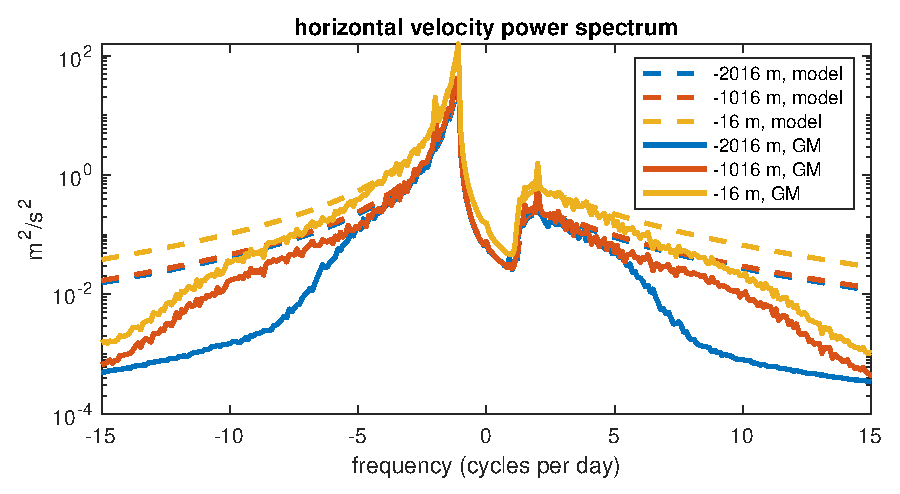
\includegraphics[width=39pc,angle=0]{figures/HorizontalVelocitySpectrum}}
  \caption{Horizontal velocity spectrum from the nonlinear steady-state run, at three different depths. The Garrett-Munk reference spectrum at those same depths is draw in dashed lines.}
  \label{HorizontalVelocitySpectrum}
\end{figure*}

%%%%%%%%%%%%%%%%%%%%%%
%
\section{Nonlinearity}
%
%%%%%%%%%%%%%%%%%%%%%%

To assess the nonlinearity of the simulations we project the dynamical variables $u$, $v$, $w$, and $\rho^\prime$ onto the linear solution at each time. This projection is exact and complete in the sense that all energy is accounted for and the projection is unique. The projection is such that each wavenumber and mode number $(k,l,j)$ is divided into three parts: positive wave solution, negative wave solution, and vortex (geostrophic) solution.

Assuming isotropy, figure \ref{Energy-nonlinear} shows the depth-integrated energy divided between the wave and vortex components as a function of vertical mode number and horizontal wavelength. The key takeaways from figure \ref{Energy-nonlinear} are,
\begin{itemize}
    \item Wave energy decreases in mode and wavenumber, as one would expected from a Garrett-Munk spectrum.
    \item The region identified as damping delineates a region of rapid energy falloff, as one would expect.
    \item There does exist vortex energy in steady-state, and it appears to be in a region roughly bordered by the Rossby radius for each mode.
    \item Outside of the damping region, the energy in these model runs is almost entirely waves. Only in low mode, high wavenumber region does there appear to be any significant fraction of energy in vortices, but only as much as 0.1\%.
\end{itemize}

\begin{figure*}[t]
  \centerline{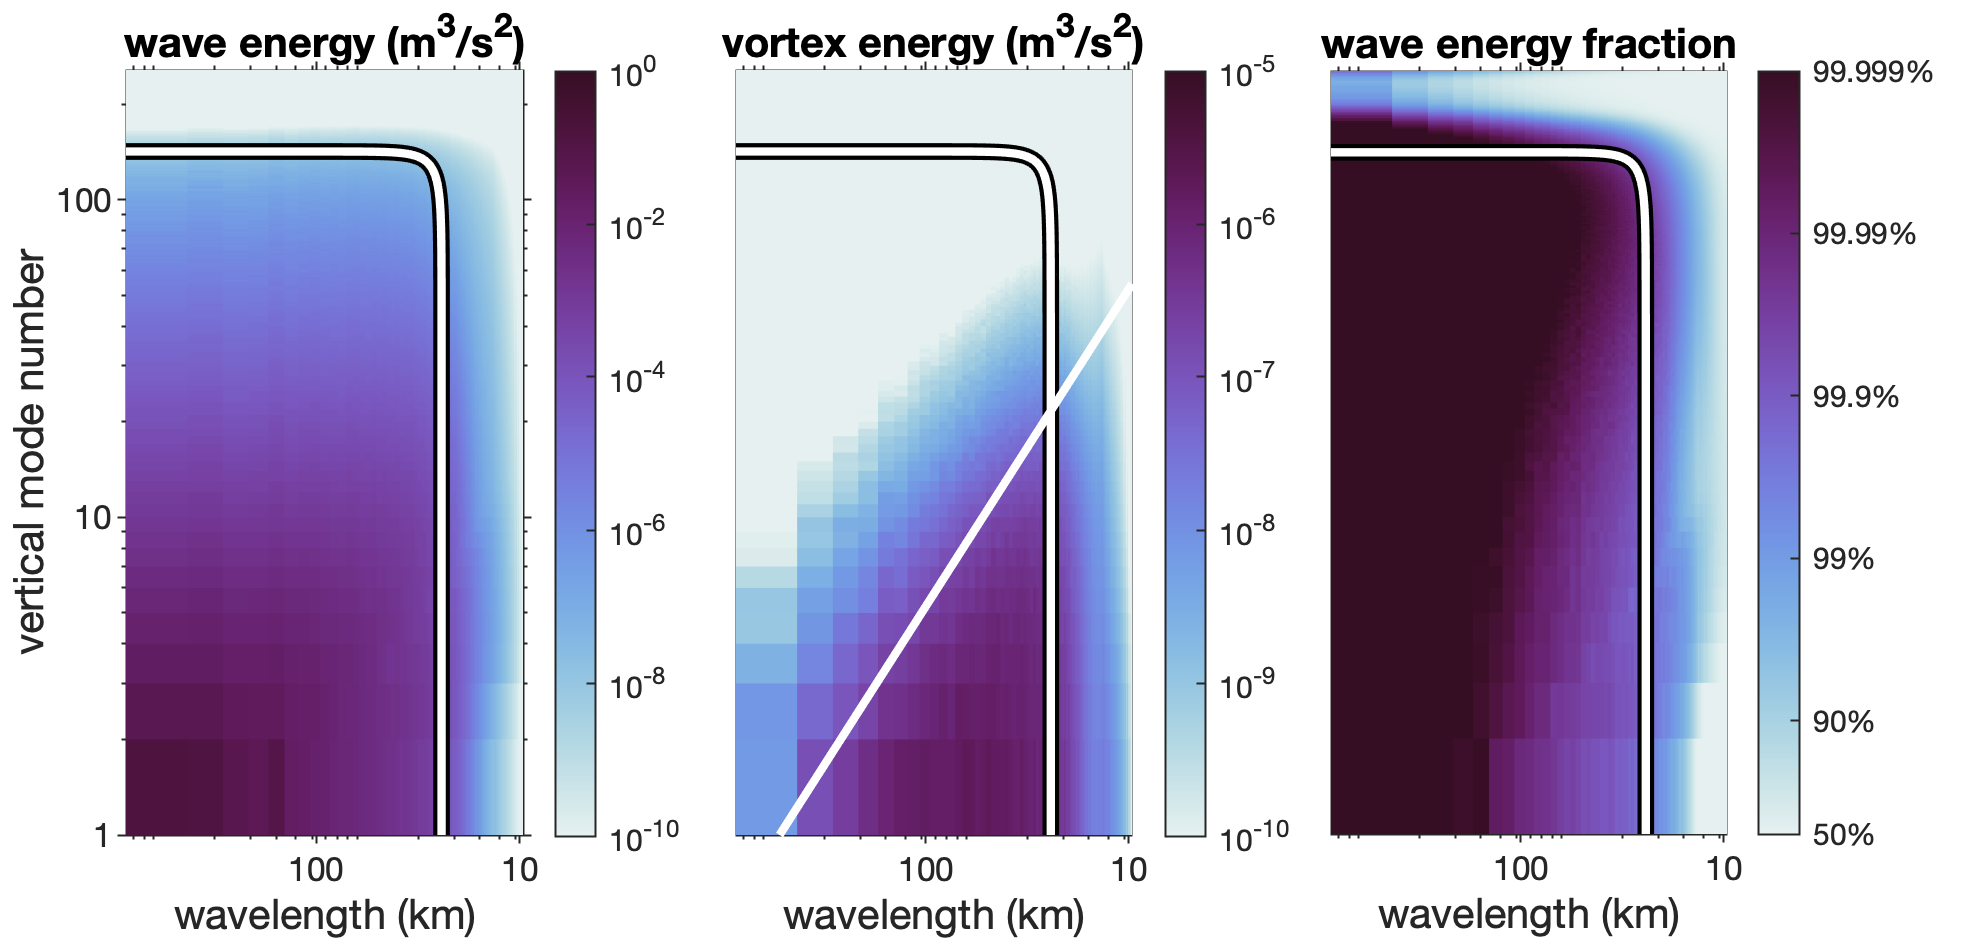
\includegraphics[width=39pc,angle=0]{figures/EnergyAndEnergyFraction-nonlinear}}
  \caption{Total depth integrated energy for the nonlinear run separated into wave and vortex components. The white contour separates the region affected by damping. The Rossby radius is drawn in white on the vortex plot. Notice the different scales in the two plots. The third panel shows the fraction of total energy that is in the wave component.}
  \label{Energy-nonlinear}
\end{figure*}

The primary reason for doing the wave-vortex decomposition is that it allows us to assess how linear or nonlinear the model is behaving. Performing the wave-vortex decomposition on the linear model run results in coefficients that remain perfectly constant in time (other than the effects of damping). This mean that any time variation of the wave-vortex coefficients from the nonlinear run, must be the result of nonlinearity.

Figures \ref{Autocorrelation_k_8_j_2} and \ref{Autocorrelation_k_12_j_228} show the value of five wave coefficients over time. The particle wave coefficients shown are chosen at random, but from two different regions in wavenumber space. In particular, figure \ref{Autocorrelation_k_8_j_2} shows coefficients from low mode and wavenumber, while figure  \ref{Autocorrelation_k_12_j_228} shows wave coefficients from a high vertical mode region. The key takeaways are,
\begin{itemize}
    \item Wave coefficients vary \emph{around} some mean value.
    \item An alternative possibility for weak nonlinearity would be that the coefficients slowly decorrelate (drift away) from their previous value.
    \item So the effects of nonlinearity are rapid (short time scale), but oscillate around a linear mean.
    \item This is seen by a rapid drop in the autocorrelation sequence, but then flatlining (rather than slowly decaying autocorrelation sequence).
    \item Near the more obviously nonlinear regions, the variance of the coefficient is larger than its mean.
\end{itemize}

\begin{figure}[t]
  \centerline{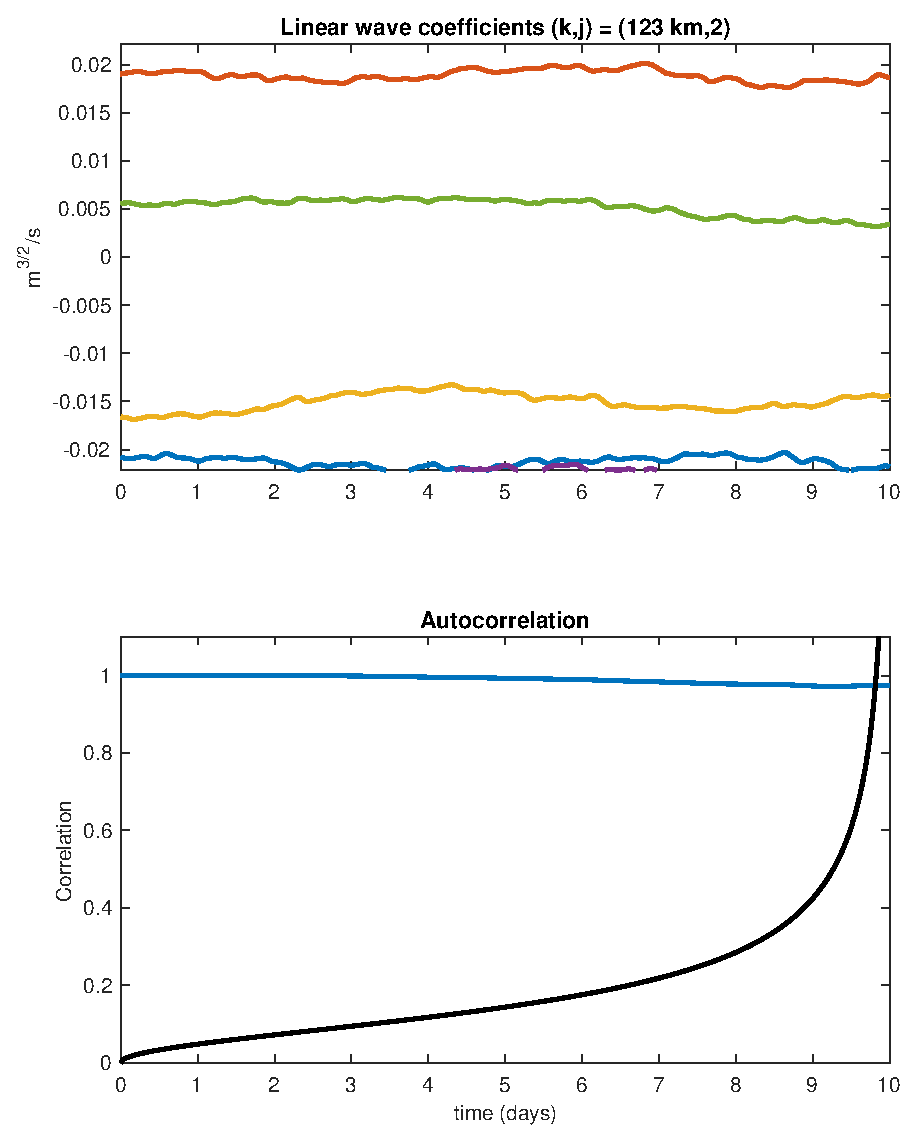
\includegraphics[width=19pc,angle=0]{figures/Autocorrelation_k_8_j_2}}
  \caption{Example linear wave components as a time series (top). The autocorrelation function of all linear wave components in that band. The standard error is drawn in black.}
  \label{Autocorrelation_k_8_j_2}
\end{figure}

\begin{figure}[t]
  \centerline{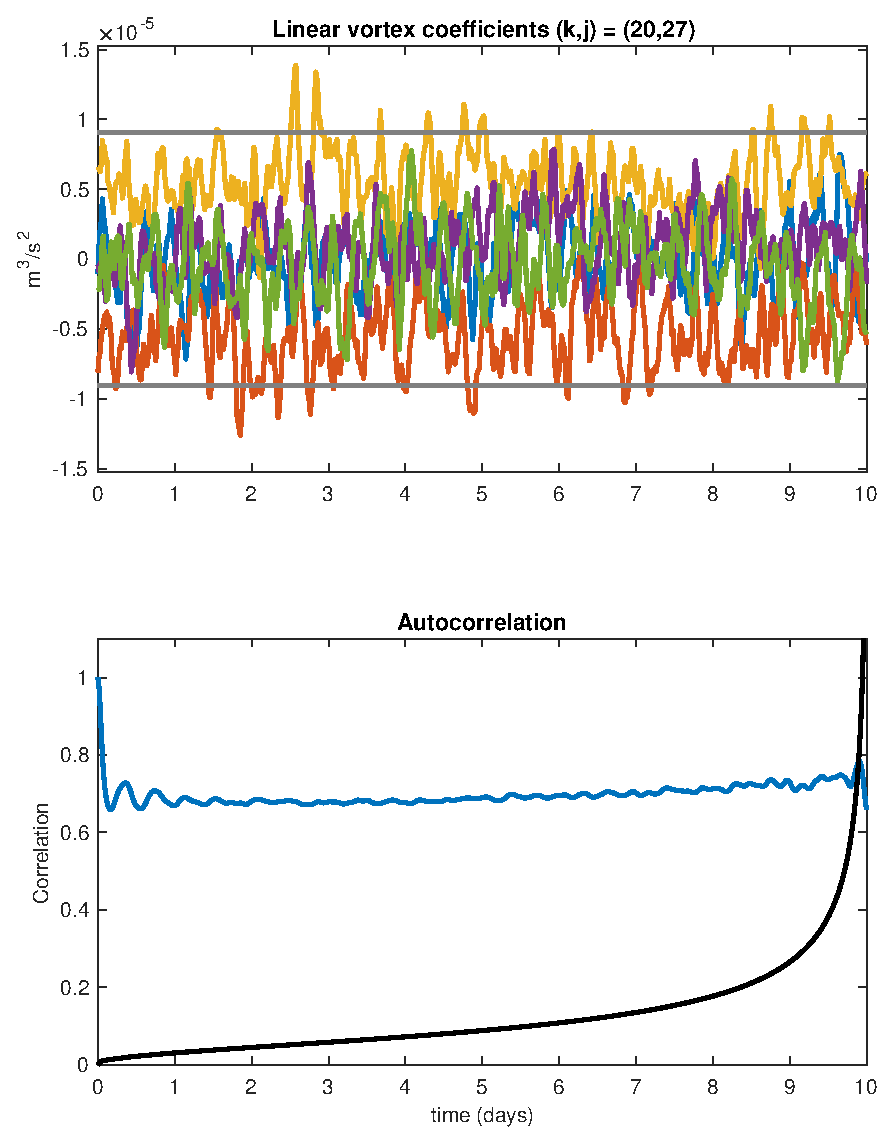
\includegraphics[width=19pc,angle=0]{figures/Autocorrelation_k_20_j_27}}
  \caption{Example linear wave components as a time series (top). The autocorrelation function of all linear wave components in that band. The standard error is drawn in black.}
  \label{Autocorrelation_k_20_j_27}
\end{figure}

\begin{figure}[t]
  \centerline{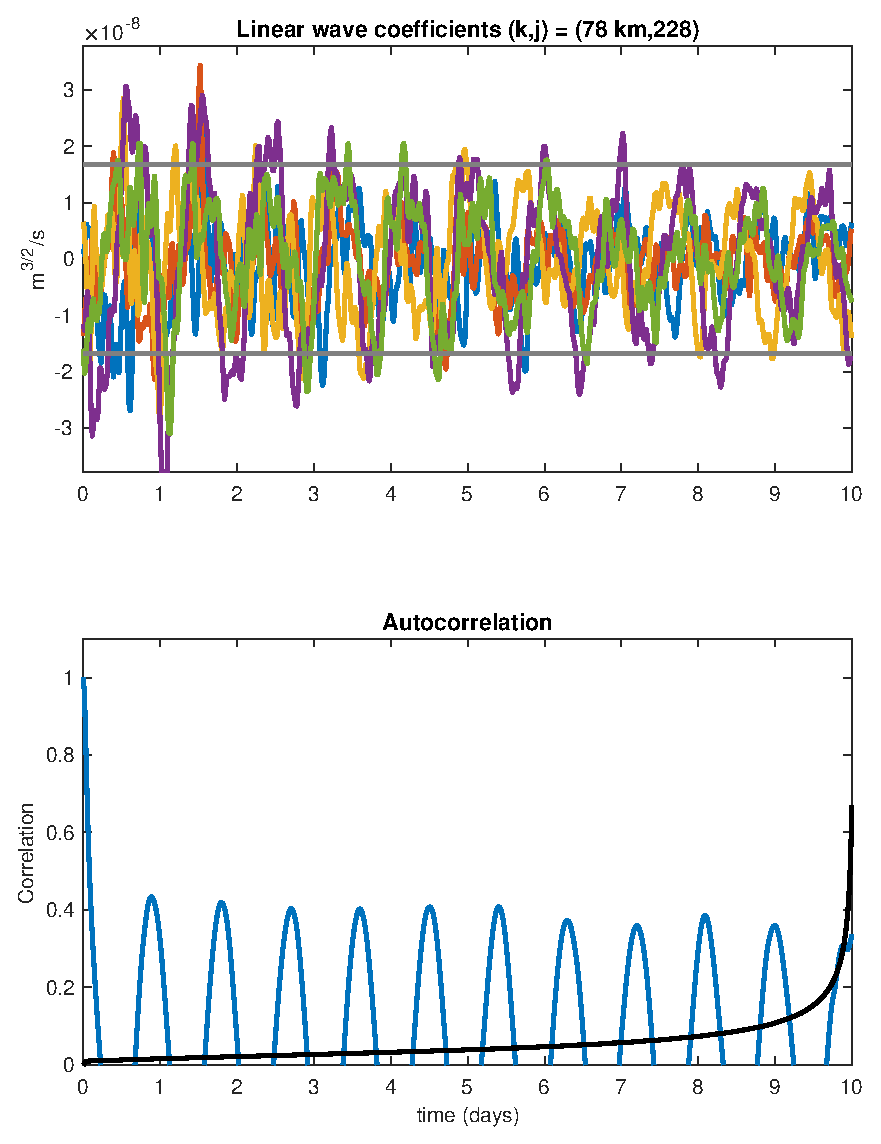
\includegraphics[width=19pc,angle=0]{figures/Autocorrelation_k_12_j_228}}
  \caption{Example linear wave components as a time series (top). The autocorrelation function of all linear wave components in that band. The standard error is drawn in black.}
  \label{Autocorrelation_k_12_j_228}
\end{figure}

We can construct a measure of nonlinearity. The time average energy for each coefficient can be divided into the time mean plus the variance over time. For a linear model run, there will be no variance in each coefficient (because the coefficients remain constant). Thus, a reasonable measure of nonlinearity is to take the ratio of the variance over time to the mean of the total energy,
\begin{equation}
    NL = \frac{\frac{1}{N_T}\sum \left( u -  \bar{u} \right)^2}{\frac{1}{N_T}\sum u^2}.
\end{equation}
This measure will give you exactly $0$ in the case of the linear model run, and exactly $1$ if the linear wave solution has no predictive power. Note that this measure of nonlinear works well \emph{given the known autocorrelation function} of the wave-vortex coefficients.

Figure \ref{WaveNonlinearity} shows the nonlinearity for the wave and vortex components. Key takeaways are,
\begin{itemize}
    \item The waves are largely linear outside of the damping region.
    \item There are hints of nonlinearity at high vertical wavenumber, and below the Rossby radius line. Which is cool!
    \item Vortices are fairly nonlinear. The linear solution still has some predictive power outside the damping region (explaining roughly half the total variance).
\end{itemize}

\begin{figure}[t]
  \centerline{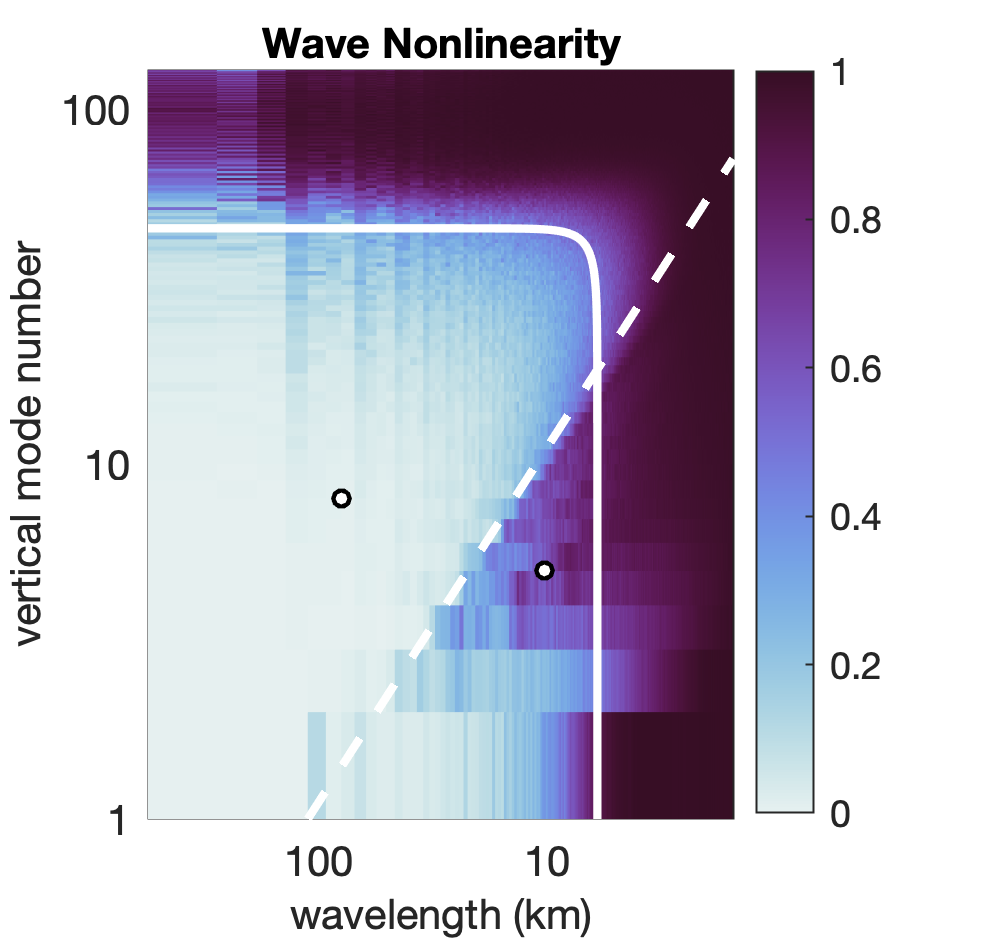
\includegraphics[width=19pc,angle=0]{figures/WaveNonlinearity}}
  \caption{Ratio of the variance around the linear mean to the total variance.}
  \label{WaveNonlinearity}
\end{figure}

\begin{figure}[t]
  \centerline{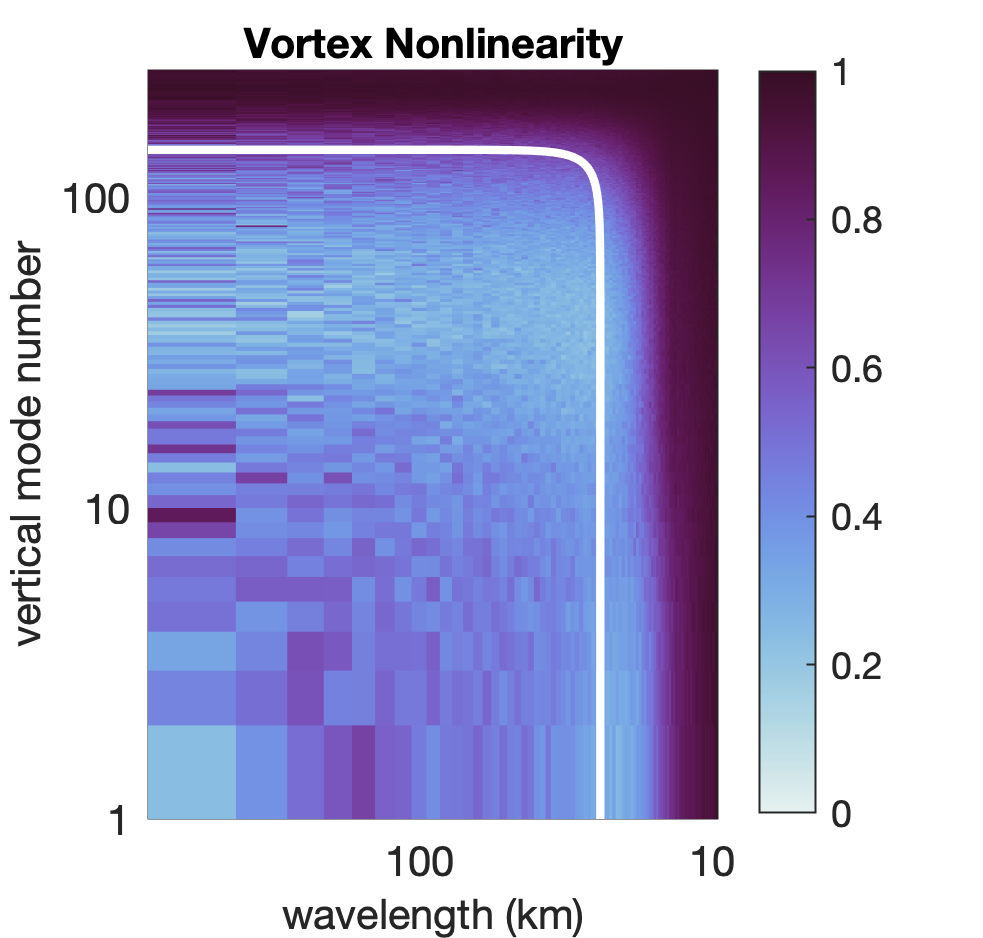
\includegraphics[width=19pc,angle=0]{figures/VortexNonlinearity}}
  \caption{Ratio of the variance around the linear mean to the total variance.}
  \label{VortexNonlinearity}
\end{figure}

%%%%%%%%%%%%%%%%%%%%%%
%
\section{Diffusivity}
%
%%%%%%%%%%%%%%%%%%%%%%

Figure \ref{DiffusivityVsScaleLinNonlin} shows the relative diffusivity of particles at different scale for the linear run (top) and nonlinear run (bottom). Key takeaways are,
\begin{itemize}
    \item Linear and nonlinear diffusivities are indistinguishable (within statistical significance).
    \item Horizontal diffusivity is greatest at the ocean boundaries.
    \item Relatively diffusivity increases with scale.
\end{itemize}

\begin{figure*}[t]
  \centerline{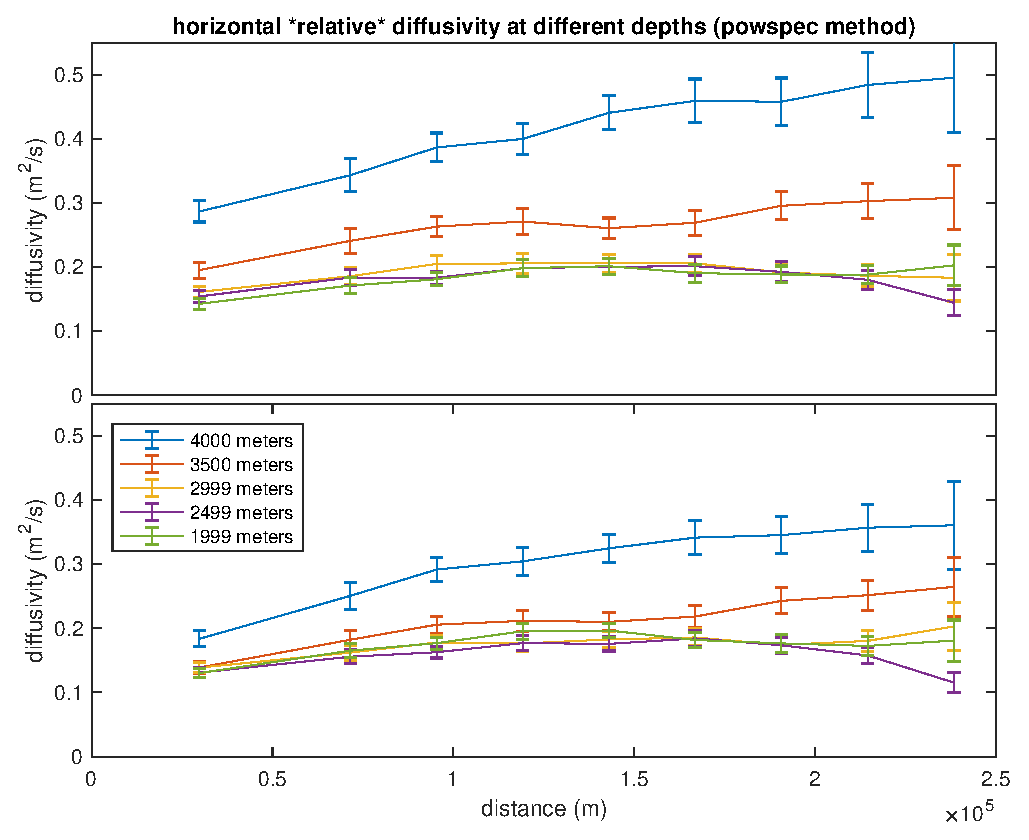
\includegraphics[width=39pc,angle=0]{figures/DiffusivityVsScaleLinNonlin}}
  \caption{Horizontal relative diffusivity as a function of spatial separation.}
  \label{DiffusivityVsScaleLinNonlin}
\end{figure*}

%% Create a bibliography directory and place your .bib file there.
%% -REMOVE ALL DIRECTORY PATHS TO REFERENCE FILES BEFORE SUBMITTING TO THE AMS FOR PEER REVIEW
\ifthenelse{\boolean{dc}}
{}
{\clearpage}
\bibliographystyle{ametsoc}
\bibliography{references}

%%%%%%%%%%%%%%%%%%%%%%%%%%%%%%%%%%%%%%%%%%%%%%%%%%%%%%%%%%%%%%%%%%%%%%
%% FIGURES-REMOVE ALL DIRECTORY PATHS TO FIGURE FILES BEFORE SUBMITTING TO THE AMS FOR PEER REVIEW
%%%%%%%%%%%%%%%%%%%%%%%%%%%%%%%%%%%%%%%%%%%%%%%%%%%%%%%%%%%%%%%%%%%%%%
%\begin{figure}[t]
%  \noindent\includegraphics[width=19pc,angle=0]{figure01.pdf}\\
%  \caption{Enter the caption for your figure here.  Repeat as
%  necessary for each of your figures. Figure from \protect\cite{Knutti2008}.}\label{f1}
%\end{figure}
%%%%%%%%%%%%%%%%%%%%%%%%%%%%%%%%%%%%%%%%%%%%%%%%%%%%%%%%%%%%%%%%%%%%%%
%% TABLES
%%%%%%%%%%%%%%%%%%%%%%%%%%%%%%%%%%%%%%%%%%%%%%%%%%%%%%%%%%%%%%%%%%%%%%
%\begin{table}[t]
%\caption{This is a sample table caption and table layout.  Enter as many tables as
%  necessary at the end of your manuscript. Table from Lorenz (1963).}\label{t1}
%\begin{center}
%\begin{tabular}{ccccrrcrc}
%\hline\hline
%$N$ & $X$ & $Y$ & $Z$\\
%\hline
% 0000 & 0000 & 0010 & 0000 \\
% 0005 & 0004 & 0012 & 0000 \\
% 0010 & 0009 & 0020 & 0000 \\
% 0015 & 0016 & 0036 & 0002 \\
% 0020 & 0030 & 0066 & 0007 \\
% 0025 & 0054 & 0115 & 0024 \\
%\hline
%\end{tabular}
%\end{center}
%\end{table}
%
\end{document}